\def \secname {Solution of non-linear equations (Root finding)}

\section[\secname]{\hyperlink{toc}{\secname}}

\begin{itemize}
    \item Consider two cases 
    \begin{enumerate}
        \item \[f(x) = 0 \qquad \text{1-D}\]
        \item \[ f(x) = 0 \qquad \text{d-D}\]
    \end{enumerate}
\end{itemize}

\subsection{ Solving nonlinear equations in one variable}

\begin{itemize}
    \item Two techniques: both presuppose info about location of root.

    \begin{enumerate}
        \item Bisection (Binary search)
        \item Newton's Method (Newton-Raphson)
    \end{enumerate}
\end{itemize}

\subsubsection{Preliminaries}

\begin{itemize}
    \item Want to find one or more roots of 

    \begin{equation}
        f(x) = 0
    \end{equation}

    \textbf{ANY} nonlinear equation can be cast in this \textbf{Canonical} form

    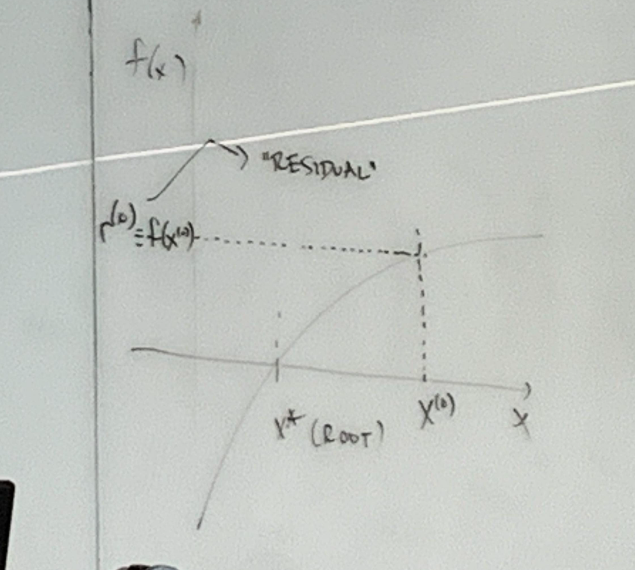
\includegraphics[width = \linewidth]{Images/410Notes_Residual.png}
    
\end{itemize}

Definition: Given Canonical equation $f(x)=0$, residual of that equation for any value x is simply $r = f(x)$

\begin{itemize}
    \item Iterative technique

    \[ x^{(0)} \rightarrow x^{(1)} \rightarrow ... \rightarrow x^{(n)} \rightarrow x^{(n+1)} \rightarrow ... \rightarrow x^{(\infty)} = x^*\]

    \[ f(x^{(0)}) \rightarrow ... \rightarrow 0 = 0\]

    \[ r^{(0)} \rightarrow ... \rightarrow 0 = 0 \]


    \item \textbf{Convergence:} Driving residual to $0\equiv$ Locating a root, $x^*$.

    \item Convergence: When do we stope iteration?

    \item Stop when
    \begin{equation}
        |\delta x^{(n)}| \equiv |x^{(n+1)} - x^{(n)}| \leq \epsilon
    \end{equation}

    for $\epsilon$ is some prescribed convergence criterion

    \item Better idea: Use relativized estimate
    
    \begin{equation}
        \frac{|\delta x^{(n)}|}{|x^{(n+1)} \leq \epsilon|}
    \end{equation}

    \item Switch over to absolute tolerance if $|x^{(n+1)}|$ becomes "too small"
    \item Motivation: Small numbers often result from "unstable" processes
\end{itemize}

\subsubsection{Bisection}

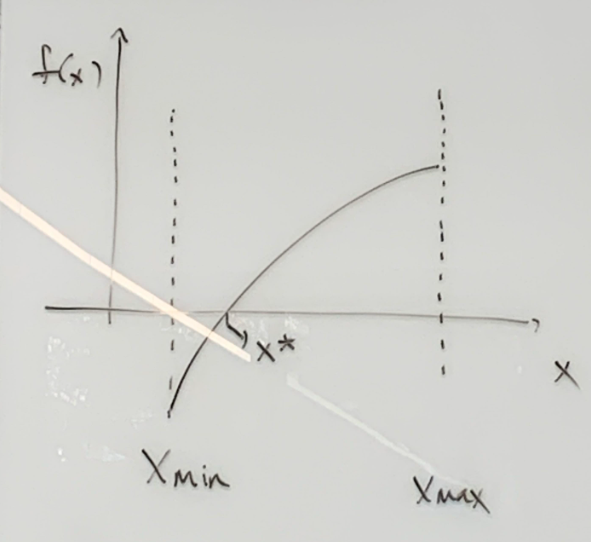
\includegraphics[width = 0.3 \linewidth]{Images/410Notes_Bisection.png}

\begin{itemize}
    \item \textbf{Demand} that $[x_{min}, w_{max}]$ contains precisely one root
    \item Demand that 
    \[f(x_{min}) f(x_{max}) < 0\]

    \item Start with initial bracket $[x_{min}, x_{max}] \rightarrow \delta x_0 = x_{max}-x_{min}$

    Generate a series of brackets with widths

    \[\delta x_1 = \delta x_0 /2 \]

    \[ \delta x_2 = \delta x_0 / 4 \]

    \[...\]

    \item Pseudocode (pseudo-MATLAB) - Can use for HW but cite

    \begin{itemize}
        \item  
        
        converged = false
        fmin = f(xmin)
        while not converged do
            xmid = (xmin+xmax)/2
            fmid = f(xmid)
            if fmid == 0
                converged = true
            elseif fmid*fmin < 0
                xmax = xmid
            else 
                xmin = xmid
                fmin = fmid
            end if 


            if (xmax-xmin)/abs(xmid) < epsilon
                converge = true
            end if 

            end while
            rout = xmid

            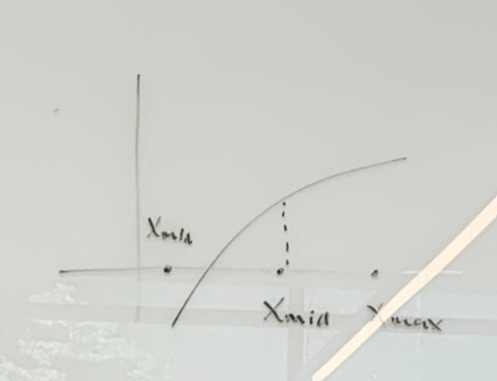
\includegraphics[width = 0.4\linewidth]{Images/410Notes_MATLAB.png}
            
        
    \end{itemize}
    \item After the l-th bisection the width of the search interval is 

    \[ \delta x_l = \delta x_0 2^ {-l} = \frac{x_{max} - x_{min}}{2^l}\]

    This is the upper bound on error in the root estimate

    
\end{itemize}

This is called divide and conquer! 
